\documentclass{beamer}
\usepackage[utf8]{inputenc}

\usetheme{Madrid}
\usecolortheme{default}
\usepackage{amsmath,amssymb,amsfonts,amsthm}
\usepackage{txfonts}
\usepackage{tkz-euclide}
\usepackage{listings}
\usepackage{adjustbox}
\usepackage{array}
\usepackage{tabularx}
\usepackage{gvv}
\usepackage{lmodern}
\usepackage{circuitikz}
\usepackage{tikz}
\usepackage{graphicx}

\setbeamertemplate{page number in head/foot}[totalframenumber]

\usepackage{tcolorbox}
\tcbuselibrary{minted,breakable,xparse,skins}



\definecolor{bg}{gray}{0.95}
\DeclareTCBListing{mintedbox}{O{}m!O{}}{%
  breakable=true,
  listing engine=minted,
  listing only,
  minted language=#2,
  minted style=default,
  minted options={%
    linenos,
    gobble=0,
    breaklines=true,
    breakafter=,,
    fontsize=\small,
    numbersep=8pt,
    #1},
  boxsep=0pt,
  left skip=0pt,
  right skip=0pt,
  left=25pt,
  right=0pt,
  top=3pt,
  bottom=3pt,
  arc=5pt,
  leftrule=0pt,
  rightrule=0pt,
  bottomrule=2pt,

  colback=bg,
  colframe=orange!70,
  enhanced,
  overlay={%
    \begin{tcbclipinterior}
    \fill[orange!20!white] (frame.south west) rectangle ([xshift=20pt]frame.north west);
    \end{tcbclipinterior}},
  #3,
}
\lstset{
    language=C,
    basicstyle=\ttfamily\small,
    keywordstyle=\color{blue},
    stringstyle=\color{orange},
    commentstyle=\color{green!60!black},
    numbers=left,
    numberstyle=\tiny\color{gray},
    breaklines=true,
    showstringspaces=false,
}
%------------------------------------------------------------
%This block of code defines the information to appear in the
%Title page
\title %optional
{1.10.28}
\date{August  2025}
%\subtitle{A short story}

\author % (optional)
{Namaswi - EE25BTECH11060}



\begin{document}


\frame{\titlepage}
\begin{frame}{Question}
Write a unit vector in \textbf{XY} plane making an angle 30\degree with positive direction of \textbf{X} axis
\end{frame}
 
\begin{frame}{given data}
\begin{table}[ht]
\centering
\begin{tabular}{|c|c|}
\hline
\textbf{Axis} & \textbf{Angle (in degrees)} \\
\hline
X-axis & 30° \\
Y-axis & 60° \\
Z-axis & 0° \\
\hline
\end{tabular}
\caption{Angles made by the X, Y, Z axes}
\end{table}

 Angle made by the vector with \textbf{X} axis = 30\degree\\
Angle made by the vector with \textbf{Y} axis =90\degree-30\degree=60\degree\\
Angle made by the vector with \textbf{Z} axis =90\degree\\
\end{frame}
\begin{frame}{Unit vector}
 Unit vector is given by 
\begin{align*}
\implies
    \begin{myvec}{\cos30\degree\\\cos60\degree\\\cos90\degree}\end{myvec}\\
    \implies
    \begin{myvec}
       {\frac{\sqrt3}{2}\\\frac{1}{2}\\0}
    \end{myvec}
\end{align*}

 
 The unit  vector of the given vector is given by
 $\frac{\sqrt{3}}{2}\,\mathbf{i} + \frac{1}{2}\,\mathbf{j}$


\end{frame}

\begin{frame}[fragile]
    \frametitle{Python Code}
    \begin{lstlisting}
 import matplotlib.pyplot as plt
import numpy as np

# Angle in radians
theta = np.deg2rad(30)

# Components of the unit vector
x = np.cos(theta)
y = np.sin(theta)

\end{lstlisting}
\end{frame}

\begin{frame}[fragile]
    \frametitle{Python Code}

    \begin{lstlisting}
    
# Plot settings
plt.figure(figsize=(5,5))
plt.axhline(0, color='black', linewidth=0.5)
plt.axvline(0, color='black', linewidth=0.5)

# Draw the unit vector
plt.quiver(0, 0, x, y, angles='xy', scale_units='xy', scale=1, color='r')
 

    \end{lstlisting}
\end{frame}

\begin{frame}[fragile]
    \frametitle{Python Code}

    \begin{lstlisting}
 # Set axis limits
plt.xlim(-0.2, 1.2)
plt.ylim(-0.2, 1.2)

# Labels
plt.text(x/2, y/2, r'$\frac{\sqrt{3}}{2}\hat{i} + \frac{1}{2}\hat{j}$', fontsize=12, color='blue')
plt.title("Unit Vector at 30° with X-axis")
plt.gca().set_aspect('equal')

plt.show()



    \end{lstlisting}
\end{frame}

 
\begin{frame}[fragile]
\frametitle{C Code}
\begin{lstlisting}
  
 #include <stdio.h>
#include <math.h>
int main() {
    double angle = 30.0;
    double angle_rad = angle * M_PI / 180.0;
    double x_component = cos(angle_rad);
    double y_component = sin(angle_rad);
    printf("Unit vector in the XY plane making a 30 degree angle with the X-axis: \n");
    printf("r = %.2f i + %.2f j\n", x_component, y_component);
    return 0;
}

\end{lstlisting}
\end{frame}

\begin{frame}[fragile]
\frametitle{Python and C Code}

\begin{lstlisting}
 import subprocess

# Compile the C program
subprocess.run(["gcc", "points.c", "-o", "points"])

# Run the compiled C program
result = subprocess.run(["./points"], capture_output=True, text=True)

# Print the output from the C program (solution steps)
print(result.stdout) 

\end{lstlisting}

\end{frame}

 \begin{figure}
    \centering
    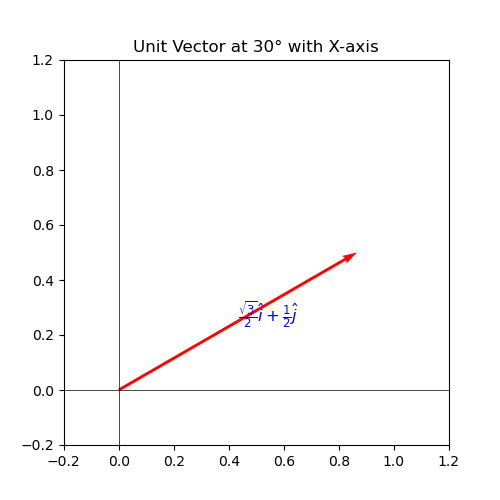
\includegraphics[width=0.8\columnwidth]{Figure _2.png}
    \caption{Plot}
    \label{fig:placeholder}
\end{figure}
\end{document}

